\documentclass{standalone}
%
\usepackage{tikz}
\usetikzlibrary{backgrounds}
\usepackage{tkz-euclide}
%
\usepackage{xcolor}
%
\definecolor{space}{HTML}{1F2C4E}
\definecolor{moon}{HTML}{AFAFAF}
\definecolor{craterm}{HTML}{616060}
\definecolor{linem}{HTML}{DBDBDB}
\definecolor{earth}{HTML}{0089FA}
\definecolor{startrek}{HTML}{F8FF00}
%
\usepackage{fontspec}
\setmainfont{Edge of the Galaxy Italic}
%
\title{A comet}
\begin{document}
	\tikzset{
		partial ellipse/.style args = {#1:#2:#3}{insert path={+ (#1:#3) arc (#1:#2:#3)}},
	}
	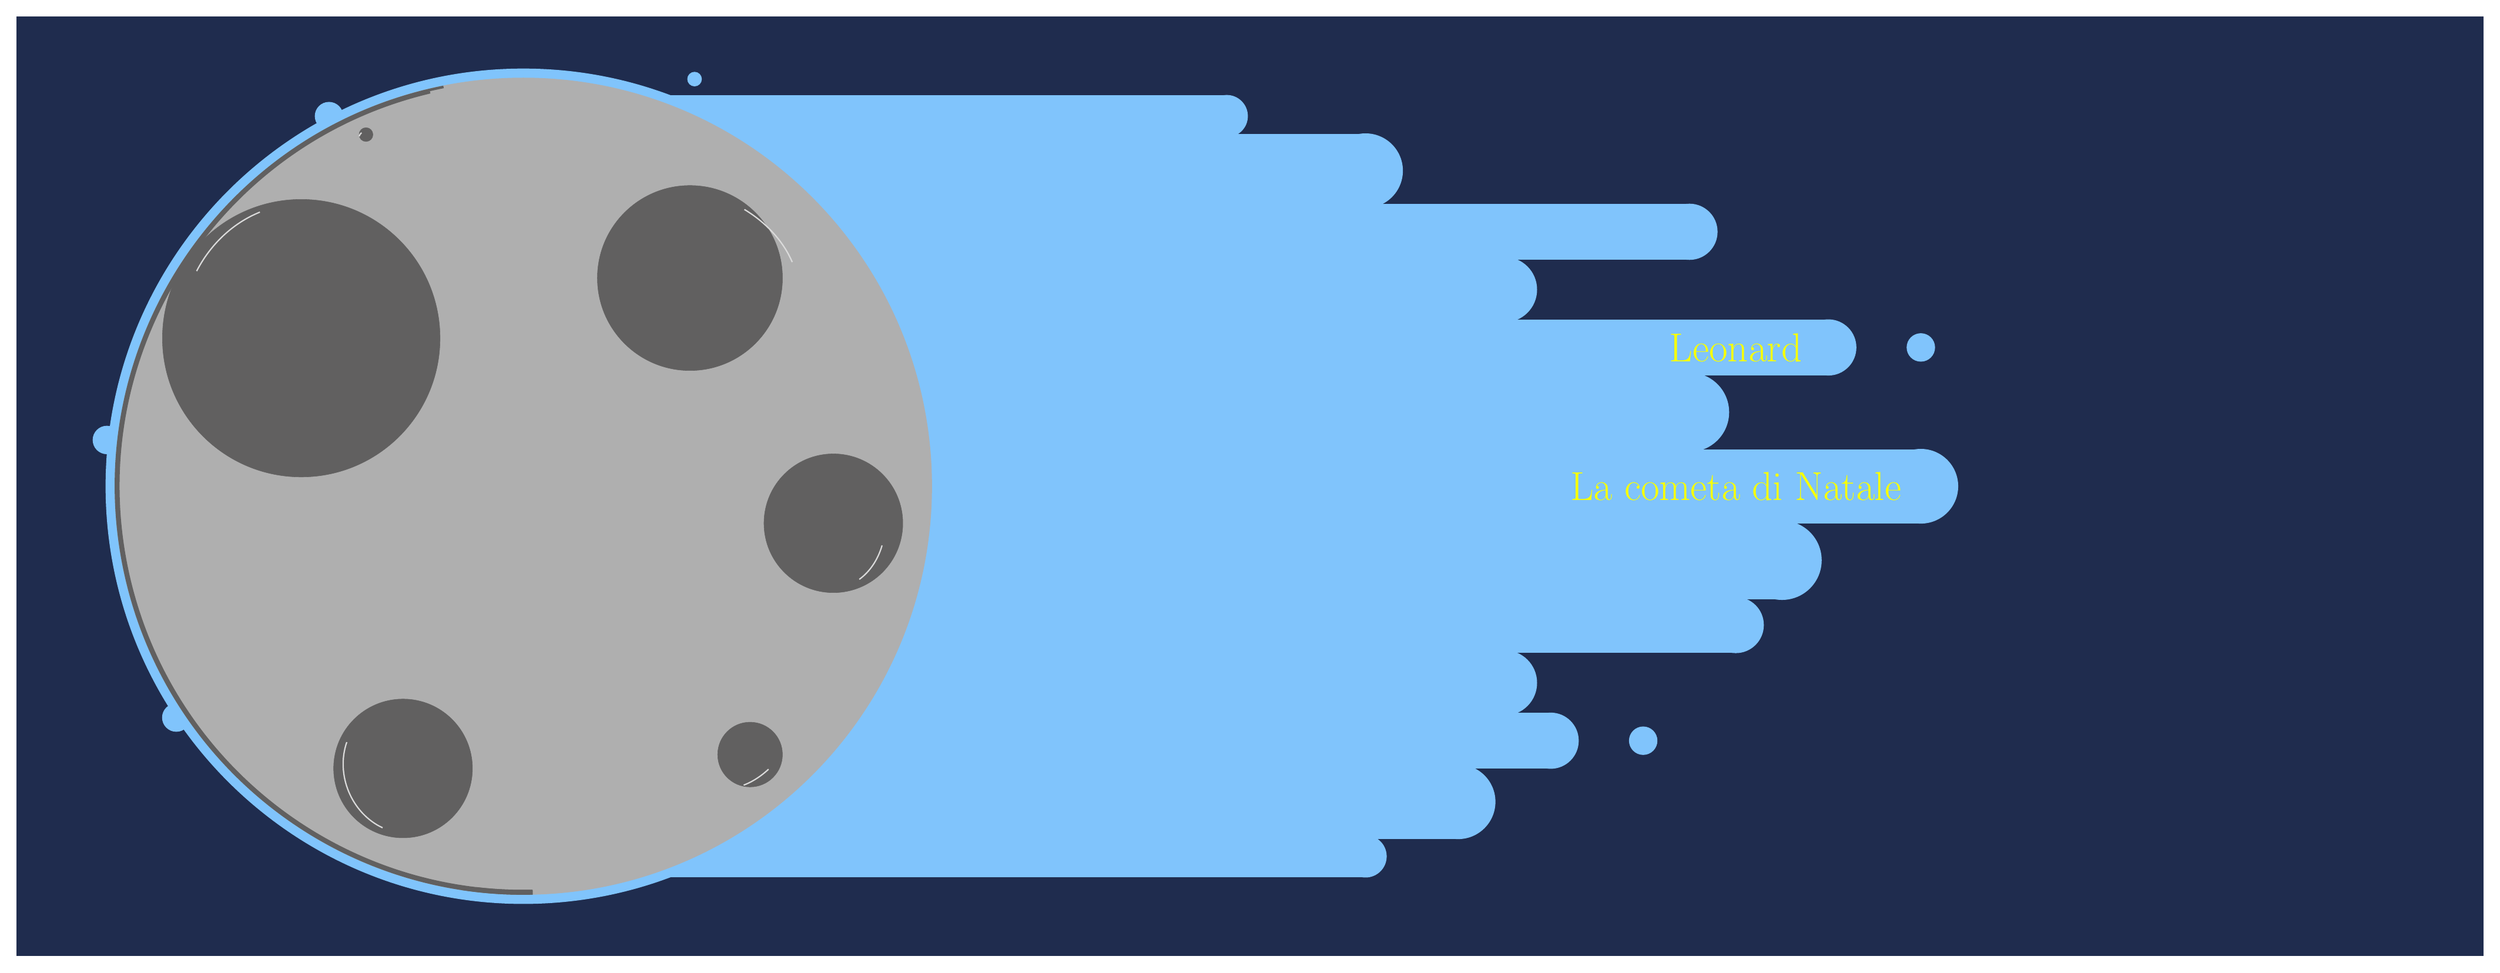
\begin{tikzpicture}[background rectangle/.style={fill=space},show background rectangle]
		%
		\draw [color=space,fill=space] (-11,-5) rectangle (42,-25);
		\begin{scope}[rotate around={-90:(0,0)}]
			\tkzDefPoint(15,-0.2){L}
			\tkzDefPoint(6.2,0){L1}
			\tkzDefPoint(15,8.8){L2}
			\tkzDefShiftPoint[L1](0:17.6){La1}
			\tkzDefShiftPoint[L1](0:17.55){La2}
			%		
			\draw [line width=16mm, color=earth!50!white] (L) -- (15,30); %center
			\draw [color=earth!50!white, fill=earth!50!white] (15,30) circle (8mm);
			\draw [line width=17mm, color=earth!50!white] (13.4,0) -- (13.4,25); %up 1
			\draw [color=earth!50!white, fill=earth!50!white] (13.4,25) circle (8.5mm);	
			\draw [line width=12mm, color=earth!50!white] (12,0) -- (12,28); %up 2
			\draw [color=earth!50!white, fill=earth!50!white] (12,28) circle (6mm);
			\draw [color=earth!50!white, fill=earth!50!white] (12,30) circle (3mm);
			\draw [line width=14mm, color=earth!50!white] (10.75,0) -- (10.75,21); %up 3
			\draw [color=earth!50!white, fill=earth!50!white] (10.75,21) circle (7mm);
			\draw [line width=12mm, color=earth!50!white] (9.5,0) -- (9.5,25); %up 4
			\draw [color=earth!50!white, fill=earth!50!white] (9.5,25) circle (6mm);
			\draw [line width=16mm, color=earth!50!white] (8.18,0) -- (8.18,18); %up 5
			\draw [color=earth!50!white, fill=earth!50!white] (8.18,18) circle (8mm);
			\draw [line width=9mm, color=earth!50!white] (7,0) -- (7,15); %up 6
			\draw [color=earth!50!white, fill=earth!50!white] (7,15) circle (4.5mm);
			\draw [line width=17mm, color=earth!50!white] (16.6,0) -- (16.6,27); %down 1
			\draw [color=earth!50!white, fill=earth!50!white] (16.6,27) circle (8.5mm);
			\draw [line width=12mm, color=earth!50!white] (18,0) -- (18,26); %down 2
			\draw [color=earth!50!white, fill=earth!50!white] (18,26) circle (6mm);
			\draw [line width=14mm, color=earth!50!white] (19.25,0) -- (19.25,21); %down 3
			\draw [color=earth!50!white, fill=earth!50!white] (19.25,21) circle (7mm);			
			\draw [line width=12mm, color=earth!50!white] (20.5,0) -- (20.5,22); %down 4
			\draw [color=earth!50!white, fill=earth!50!white] (20.5,22) circle (6mm);
			\draw [color=earth!50!white, fill=earth!50!white] (20.5,24) circle (3mm);
			\draw [line width=16mm, color=earth!50!white] (21.82,0) -- (21.82,20); %down 5
			\draw [color=earth!50!white, fill=earth!50!white] (21.82,20) circle (8mm);
			\draw [line width=9mm, color=earth!50!white] (23,0) -- (23,18); %down 6
			\draw [color=earth!50!white, fill=earth!50!white] (23,18) circle (4.5mm);
			%
			\draw [color=earth!50!white, fill=earth!50!white] (6.2,3.5) circle (1.5mm);			
			%
			\draw [color=earth!50!white, fill=earth!50!white] (7,-4.4) circle (3mm);
			\draw [color=earth!50!white, fill=earth!50!white] (14,-9.2) circle (3mm);
			\draw [color=earth!50!white, fill=earth!50!white] (20,-7.7) circle (3mm);
			\tkzDrawCircle[color=earth!50!white,fill=earth!50!white,ultra thick](L,L2)
			\tkzDrawCircle[color=moon,fill=moon,ultra thick](L,L1)
			\tkzDrawArc[ultra thick, color=craterm, rotate](L,La1)(-170)
			\tkzDrawArc[ultra thick, color=craterm, rotate](L,La1)(-10)
			\tkzDrawArc[ultra thick, color=craterm, rotate](L,La2)(-168)
			\tkzDrawArc[ultra thick, color=craterm, rotate](L,La2)(-8)
			%
			\tkzDefPoint(7.4,-3.6){M1}
			\tkzDefShiftPoint[M1](0:0.15){Mr1}
			\tkzDefShiftPoint[Mr1](0:-0.05){Ma1}
			\begin{scope}[rotate around={30:(M1)},yscale=1.8]
				\tkzDrawCircle[color=craterm,fill=craterm](M1,Mr1)
				\tkzDrawArc[rotate around={220:(M1)},thick,color=linem,rotate](M1,Ma1)(40)
			\end{scope}
			%
			\tkzDefPoint(20.8,4.7){M2}
			\tkzDefShiftPoint[M2](0:0.7){Mr2}
			\tkzDefShiftPoint[Mr2](0:-0.1){Ma2}
			\begin{scope}[rotate around={40:(M2)},yscale=1.9]
				\tkzDrawCircle[color=craterm,fill=craterm](M2,Mr2)
				\tkzDrawArc[rotate around={-10:(M2)},thick,color=linem,rotate](M2,Ma2)(40)
			\end{scope}
			%
			\tkzDefPoint(15.8,6.5){M3}
			\tkzDefShiftPoint[M3](0:1.5){Mr3}
			\tkzDefShiftPoint[Mr3](0:-0.1){Ma3}
			\begin{scope}[yscale=0.8]
				\tkzDrawCircle[color=craterm,fill=craterm](M3,Mr3)
				\tkzDrawArc[rotate around={30:(M3)},thick,color=linem,rotate](M3,Ma3)(40)
			\end{scope}
			%
			\tkzDefPoint(21.1,-2.8){M4}
			\tkzDefShiftPoint[M4](0:1.5){Mr4}
			\tkzDefShiftPoint[Mr4](0:-0.1){Ma4}
			\begin{scope}[rotate around={20:(M4)},yscale=0.9]
				\tkzDrawCircle[color=craterm,fill=craterm](M4,Mr4)
				\tkzDrawArc[rotate around={-20:(M4)},thick,color=linem,rotate](M4,Ma4)(-90)
			\end{scope}
			%
			\tkzDefPoint(11.8,-5){M6}
			\tkzDefShiftPoint[M6](0:3){Mr6}
			\tkzDefShiftPoint[Mr6](0:-0.1){Ma6}
			\begin{scope}[yscale=0.9]
				\tkzDrawCircle[color=craterm,fill=craterm](M6,Mr6)
				\tkzDrawArc[rotate around={-160:(M6)},thick,color=linem,rotate](M6,Ma6)(40)
			\end{scope}
			%
			\tkzDefPoint(10.5,3.4){M7}
			\tkzDefShiftPoint[M7](0:2){Mr7}
			\tkzDefShiftPoint[Mr7](0:-0.1){Ma7}
			\begin{scope}[rotate around={-20:(M7)},yscale=1.3]
				\tkzDrawCircle[color=craterm,fill=craterm](M7,Mr7)
				\tkzDrawArc[rotate around={110:(M7)},thick,color=linem,rotate](M7,Ma7)(40)
			\end{scope}
		\end{scope}
		%
		\node at (26,-12) {\textcolor{startrek}{\fontsize{90}{91}\selectfont Leonard}};
		\node at (26,-15) {\textcolor{startrek}{\fontsize{90}{91}\selectfont La cometa di Natale}};
	\end{tikzpicture}
\end{document}